% Báo cáo BTL1 — Nhập môn Trí tuệ nhân tạo — bản tiếng Việt.
% Dựng PDF: tectonic report/main-vi.tex
\documentclass[12pt,a4paper]{article}
% Shared packages for the standalone report and a merged team report.
\usepackage[a4paper,top=27mm,bottom=24mm,left=26mm,right=24mm,headheight=36pt,headsep=7mm]{geometry}
\usepackage{fontspec}
\IfFontExistsTF{Times New Roman}{\setmainfont{Times New Roman}}{%
\setmainfont{texgyretermes}[Extension=.otf,UprightFont=*-regular,
BoldFont=*-bold,ItalicFont=*-italic,BoldItalicFont=*-bolditalic]}
\setsansfont{lmsans10-regular.otf}[BoldFont=lmsans10-bold.otf,ItalicFont=lmsans10-oblique.otf]
\setmonofont{lmmono10-regular.otf}[Scale=0.88]
\usepackage{amsmath,amssymb,booktabs,array,tabularx,multirow}
\usepackage{graphicx,xcolor,tikz,pgfplots}
\usetikzlibrary{arrows.meta,positioning,calc,shapes.geometric}
\pgfplotsset{compat=1.18}
\usepackage{enumitem,float,caption,subcaption,listings,etoolbox}
\usepackage{fancyhdr,lastpage,setspace,microtype,needspace}
\usepackage[unicode,colorlinks=true,linkcolor=black,citecolor=black,urlcolor=blue!60!black]{hyperref}
\usepackage{bookmark}
\definecolor{pipeblue}{HTML}{285BC2}
\definecolor{water}{HTML}{258BD2}
\definecolor{muted}{HTML}{616A76}
\definecolor{reject}{HTML}{B6473C}
\renewcommand{\contentsname}{Mục lục}
\renewcommand{\figurename}{Hình}
\renewcommand{\tablename}{Bảng}
\renewcommand{\refname}{Tài liệu tham khảo}
\renewcommand{\lstlistingname}{Mã giả}
\setcounter{tocdepth}{2}
\setcounter{secnumdepth}{3}
\setstretch{1.10}
\setlength{\parindent}{1.2em}
\setlength{\parskip}{3pt}
\setlist{nosep,topsep=4pt,leftmargin=1.5em}
\captionsetup{font=small,labelfont=bf,skip=7pt}
\lstset{basicstyle=\ttfamily\small,columns=fullflexible,keepspaces=true,
  showstringspaces=false,breaklines=true,frame=single,rulecolor=\color{black!25},
  xleftmargin=1mm,xrightmargin=1mm,framesep=5pt,numbers=left,numberstyle=\tiny\color{muted},
  numbersep=9pt,aboveskip=8pt,belowskip=8pt,
  keywordstyle=\color{pipeblue},morekeywords={if,else,for,in,while,return,and,or,not,def}}
\pagestyle{fancy}
\fancyhf{}
\fancyhead[L]{\parbox[c][11mm][c]{\textwidth}{\normalfont\normalsize
  \parbox[c]{11mm}{
\includegraphics[height=10mm]{assets/hcmut-logo.png}}\hspace{4mm}%
  \parbox[c]{.85\textwidth}{\normalfont\fontsize{8.5}{10.5}\selectfont
  TRƯỜNG ĐẠI HỌC BÁCH KHOA - ĐHQG TP.HCM\\
  KHOA KHOA HỌC VÀ KỸ THUẬT MÁY TÍNH}}}
\fancyfoot[L]{\fontsize{8}{10}\selectfont BTL Nhập môn Trí tuệ nhân tạo - Học kỳ 261}
\fancyfoot[R]{\fontsize{8}{10}\selectfont Trang \thepage/\pageref*{LastPage}}
\renewcommand{\headrulewidth}{.4pt}
\renewcommand{\footrulewidth}{.4pt}
\newcommand{\code}[1]{\texttt{\detokenize{#1}}}
\newcommand{\R}{\mathcal{R}}
\newcommand{\D}{\mathcal{D}}
\newcommand{\pipetile}[4]{%
\begin{scope}[shift={(#1,#2)}]
  \draw[black!18] (-.5,-.5) rectangle (.5,.5);
  \foreach \bit/\dx/\dy in {1/0/.5,2/.5/0,4/0/-.5,8/-.5/0}{%
    \pgfmathtruncatemacro{\hasport}{mod(floor(#3/\bit),2)}
    \ifnum\hasport=1\draw[#4,line width=3pt,line cap=round] (0,0)--(\dx,\dy);\fi}
\end{scope}}
\newcommand{\pipeboard}[2]{%
\foreach \mask[count=\idx from 0] in {#1}{%
  \pgfmathtruncatemacro{\col}{mod(\idx,4)}
  \pgfmathtruncatemacro{\row}{-floor(\idx/4)}
  \pipetile{\col}{\row}{\mask}{#2}}
\fill[white] (2,-2) circle (.16);\fill[pipeblue] (2,-2) circle (.105);}

% Fill in current team details before submission. Do not reuse the sample's authors.
\newcommand{\CourseName}{INTRODUCTION TO ARTIFICIAL INTELLIGENCE}
\newcommand{\CourseCode}{CO3061}
\newcommand{\Semester}{261}
\newcommand{\ReportMonth}{Tháng 10 năm 2026}
\newcommand{\InstructorName}{Ths. Vương Bá Thịnh}
% Example: Họ tên thứ nhất & MSSV thứ nhất & Lớp thứ nhất \\ Họ tên thứ hai & MSSV thứ hai & Lớp thứ hai
\newcommand{\StudentRows}{Hà Bảo Nhi & 2312496 & (L01) \\ Lê Chí Đại & 2310621 & (L01) \\ Đào Quang Dương & 2310579 & (L01) \\ Lương Minh Thuận & 2313348 & (L02) \\ Nguyễn Quốc Huy & 2311209 & (L02)}

\hypersetup{pdftitle={BTL1 - Tìm kiếm: Pipes và Light Up},
  pdfsubject={DFS, Greedy Best-First và Backtracking với MRV/CP}}

\definecolor{codekw}{HTML}{285BC2}
\lstset{basicstyle=\ttfamily\small,columns=fullflexible,keepspaces=true,
  showstringspaces=false,keywordstyle=\color{codekw},frame=single,
  rulecolor=\color{gray!40},framerule=0.3pt,aboveskip=8pt,belowskip=8pt,breaklines=true}

\captionsetup{font=small,labelfont=bf}
\setlength{\parskip}{2pt}
\setlength{\emergencystretch}{3em}

\renewcommand{\code}[1]{\texttt{#1}}
\definecolor{ink}{HTML}{25282D}

\begin{document}
\hypersetup{pageanchor=false}

% ---------- Trang bìa ----------
\begin{titlepage}
\centering
\vspace*{10mm}
{\large ĐẠI HỌC QUỐC GIA THÀNH PHỐ HỒ CHÍ MINH\\[2mm]
TRƯỜNG ĐẠI HỌC BÁCH KHOA\\[2mm]
KHOA KHOA HỌC VÀ KỸ THUẬT MÁY TÍNH\par}
\vspace{10mm}
\includegraphics[height=30mm]{assets/hcmut-logo.png}\par
\vspace{17mm}
{\Large\bfseries INTRODUCTION TO\\[2mm]ARTIFICIAL INTELLIGENCE (\CourseCode)\par}
\vspace{6mm}\hrule\vspace{5mm}
{\Large\bfseries BÁO CÁO BÀI TẬP LỚN 1\par}
\vspace{5mm}{\Large\bfseries TÌM KIẾM (SEARCHING)\par}
\vspace{4mm}{\large Pipes và Light Up (Akari)\par}
\vspace{5mm}\hrule\vspace{10mm}
\begin{minipage}{.78\textwidth}\raggedright
\ifdefempty{\InstructorName}{\textbf{Giảng viên:}\ \rule{.65\linewidth}{.2pt}\par}{\textbf{Giảng viên:} \InstructorName\par}
\vspace{3mm}
\ifdefempty{\ClassName}{\textbf{Lớp:}\ \rule{.75\linewidth}{.2pt}\par}{\textbf{Lớp:} \ClassName\par}
\vspace{4mm}\textbf{Sinh viên thực hiện:}\par\vspace{3mm}
\ifdefempty{\StudentRows}{\rule{.95\linewidth}{.2pt}\par\vspace{5mm}\rule{.95\linewidth}{.2pt}\par}{\begin{tabular}{@{}ll@{}}\StudentRows\end{tabular}}
\end{minipage}
\vfill{\normalsize THÀNH PHỐ HỒ CHÍ MINH, \ReportMonth\par}\vspace{7mm}
\end{titlepage}
\pagenumbering{arabic}
\hypersetup{pageanchor=true}
\tableofcontents
\newpage

% Phần Pipes của báo cáo — được \input từ main-vi.tex / main-en.tex.
\section{Bài toán 1: Pipes}

\subsection{Tìm hiểu đề bài và luật chơi}

Nhóm tìm hiểu Pipes qua việc chơi trực tiếp trên \url{https://www.puzzle-pipes.com/}
và quan sát hành vi của game gốc. Sau quá trình chơi thử, nhóm tóm tắt luật như sau:

\begin{itemize}
\item Bàn chơi $m\times m$ gồm các ô ống. Mỗi ô có \emph{hình dạng cố định}
(ống thẳng, khuỷu, chữ T, chữ thập, đầu cụt) và một \emph{định hướng} (hướng xoay)
có thể thay đổi; xoay là tác động duy nhất của người chơi.
\item Mỗi hình dạng có một tập cổng ở các phía Bắc--Đông--Nam--Tây. Xoay ô không
đổi số cổng, chỉ đổi hướng.
\item Mục tiêu: xoay sao cho \textbf{mọi} cổng mở đều gặp cổng mở tương ứng của ô
kề (không cổng nào chìa ra ngoài biên, không cổng nào \emph{dangling}), toàn bộ
các ô nối thành \textbf{một} mạng liên thông và mạng \textbf{không chứa chu trình}.
\item Nguồn nước (ô đánh dấu trên game gốc) chỉ để trực quan hóa: khi mạng hoàn
chỉnh, nước chảy từ nguồn tới mọi ô. Đổi vị trí nguồn không làm đổi tập các bàn
hợp lệ.
\end{itemize}

Nhìn theo phân loại của giáo trình, đây là bài toán \emph{một agent, tất định,
quan sát được toàn phần, rời rạc, tĩnh}. Đây là bài toán \emph{thỏa mãn}
(satisfaction): mọi bàn hợp lệ đều là lời giải, bài toán không yêu cầu tối ưu số
lần xoay. Trò chơi gốc cũng không tính điểm theo số bước xoay.

\subsection{Phát biểu bài toán tìm kiếm}

Gọi $n = m^2$, đánh số các ô theo thứ tự hàng--cột (row-major). Ô $i$ có hình dạng
cố định và miền định hướng $R_i$ gồm các xoay phân biệt của hình dạng đó. Nhóm
phát biểu bài toán như sau:

\begin{table}[h]
\centering\small
\begin{tabular}{@{}p{.20\textwidth}p{.74\textwidth}@{}}
\toprule
Thành phần & Định nghĩa trong cài đặt\\
\midrule
Input & Bàn chơi đã xáo trộn (hình dạng + định hướng lưu sẵn), kích thước, nguồn\\
Trạng thái & Tiền tố $s=(a_0,\dots,a_{k-1})$ các định hướng đã gán\\
Trạng thái đầu & Tiền tố rỗng $()$, biết trước toàn bộ hình dạng\\
Tác động & Gán một định hướng hợp lệ biên cho ô $k$ (ô kế tiếp theo row-major)\\
Chuyển tiếp & $s' = s + (a_k)$, chỉ nhận khi qua hết các kiểm tra khả thi\\
Kiểm tra đích & $k=n$ và bàn hoàn chỉnh thỏa mọi luật\\
Chi phí & 1 mỗi phép gán; không giải thuật nào dùng chi phí để xếp hạng\\
Lời giải & Một bộ định hướng đầy đủ hợp lệ\\
\bottomrule
\end{tabular}
\caption{Phát biểu bài toán tìm kiếm cho Pipes.}
\end{table}

Điểm cần nhấn: \emph{một bước của giải thuật} là gán \textbf{tuyệt đối} một định
hướng cho ô kế tiếp, khác với \emph{một bước của người chơi} là xoay 90 độ. Một
phép gán có thể tương ứng 0--3 lần xoay. Cả hai giải thuật dùng cùng mô hình gán,
nên việc so sánh chúng là công bằng. Nhóm cũng tách bạch trạng thái tìm kiếm
(tiền tố rỗng) với bàn xáo trộn lưu trong file input: bàn xáo trộn cung cấp miền
$R_i$ và thứ tự duyệt các xoay, còn tìm kiếm luôn bắt đầu từ tiền tố rỗng, không
dựa vào đáp án của generator.

\subsection{Không gian tìm kiếm và cắt tỉa dùng chung}

Số cách gán đầy đủ (chưa xét biên) là $U=\prod_i |R_i| \le 4^n$: ô khuỷu/T/đầu
cụt có 4 xoay phân biệt, ống thẳng có 2, ô chữ thập có 1. Với bàn 4$\times$4 điển
hình $U = 4^{16} \approx 4{,}29\times10^9$; với 7$\times$7 cận trên là
$4^{49} \approx 3{,}17\times10^{29}$. Cây gán có độ sâu $n$, hệ số phân nhánh tối
đa 4, và \textbf{mỗi tiền tố có đúng một cha} (thứ tự gán cố định), nên không cần
bảng closed để chống lặp trạng thái.

Trước khi tìm kiếm, các định hướng chìa cổng ra ngoài biên bị loại. Với mỗi ứng
viên con, hàm \code{compatible()} dùng chung cho cả hai giải thuật thực hiện ba
lớp cắt tỉa hợp lệ (sound):

\begin{enumerate}
\item \textbf{Khớp với láng giềng đã gán}: mỗi miền $R_i$ chưa gán bị thu hẹp chỉ
giữ định hướng khớp cổng của các ô đã gán (cả cổng có lẫn cổng \emph{không} có).
Miền nào rỗng thì chặn nhánh.
\item \textbf{Chặn chu trình}: nếu các ô đã gán tạo chu trình thì loại (dùng cấu
trúc disjoint-set).
\item \textbf{Kết nối khả dĩ}: dựng đồ thị \emph{lạc quan} giữa các ô — có cạnh
nếu hai ô \emph{có thể} mở cổng về phía nhau với một định hướng còn lại nào đó.
Nếu đồ thị này không liên thông thì không thể có mạng hoàn chỉnh, chặn nhánh.
\end{enumerate}

Tại gốc, kiểm tra nhanh $2(n-1)$ cổng: mạng cây trên $n$ đỉnh có đúng $n-1$ cạnh
$= 2(n-1)$ cổng; xoay không đổi số cổng nên tổng sai chứng tỏ vô nghiệm ngay từ
đầu. Điều ngược lại không đúng (đủ cổng chưa chắc có nghiệm). Cả ba lớp cắt tỉa
đều chỉ loại trạng thái \emph{không thể} dẫn tới nghiệm nên không mất tính đầy đủ.
DFS do đó là giải thuật mù về \emph{thứ tự duyệt}, nhưng vẫn là DFS có cắt tỉa
ràng buộc chứ không phải máy đếm xoay vét cạn.

\subsection{Giải thuật tìm kiếm mù: Depth-First Search}

DFS đi sâu theo nhánh con khả thi đầu tiên cho đến khi gặp đích hoặc bế tắc rồi
quay lui. Thứ tự duyệt các xoay là thứ tự lưu sẵn của từng ô — hoàn toàn không
dùng thông tin heuristic:

\begin{lstlisting}
SEARCH_DFS(input):
  build boundary-valid domains R_i
  if root feasibility fails: return UNSOLVABLE
  return VISIT(())

VISIT(s):
  if budget exhausted: return LIMIT_REACHED
  count one expansion
  if GOAL(s): return SOLVED(s)
  for a in boundary-valid rotations of tile |s|:
    child = s + (a)
    if FEASIBLE(child):           # 3 pruning layers
      r = VISIT(child)
      if r is SOLVED or LIMIT_REACHED: return r
  return UNSOLVABLE
\end{lstlisting}

Với không gian hữu hạn, cây có chu kỳ bị cắt bởi cấu trúc tiền tố, và cắt tỉa là
hợp lệ nên DFS \emph{đầy đủ} nếu đủ tài nguyên. Lời giải đầu tiên tìm được không
đảm bảo tối ưu số phép gán. Độ phức tạp thời gian xấu nhất là hàm mũ theo $n$;
về bộ nhớ, DFS giữ đường hiện hành và các nhánh chưa xét — cài đặt Python giữ bản
sao tiền tố và khung generator cho mỗi mức, khoảng $O(n^2)$ trên một nhánh.

\subsection{Giải thuật heuristic: Greedy Best-First}

Greedy luôn pop khỏi hàng ưu tiên (min-heap) trạng thái có ít \emph{lựa chọn còn
lại} nhất:
\[
h(s) = \sum_{i \text{ chưa gán}} \log_2 |D_i(s)|, \qquad
\text{priority}(s) = (h(s),\ -\text{depth}(s),\ \text{insertion order})
\]
với $D_i(s)$ là miền biên-hợp-lệ của ô $i$ sau khi khớp với các láng giềng đã
gán. Tổng là logarit của tích các miền còn lại: ví dụ miền $(1,2,4)$ cho
$h=0+1+2=3$, còn $(1,1,2)$ cho $h=1$ — trạng thái B ít ``tự do'' hơn và được ưu
tiên. Nhóm chọn heuristic này vì: (i) nó rẻ, chỉ cần miền đã tính trong bước cắt
tỉa; (ii) mọi lời giải ở cùng độ sâu đều cần đúng $n$ phép gán nên $n-k$ không
phân biệt được gì, còn tổng log-miền ưu tiên nhánh ít phân nhánh nhất. $h$ ở đây
\emph{không admissible} — nó đo độ bất định còn lại, không phải cận dưới chi phí;
và không dùng thành phần $g$.

\begin{lstlisting}
SEARCH_GREEDY(input):
  build boundary-valid domains; root feasibility check
  push () into min-priority queue with priority 0
  while queue is not empty:
    if budget exhausted: return LIMIT_REACHED
    s = pop minimum-priority state;  count one expansion
    if GOAL(s): return SOLVED(s)
    for a in boundary-valid rotations of tile |s|:
      child = s + (a);  D = FEASIBLE(child)
      if D exists: push child with (h(child), -|child|, serial)
  return UNSOLVABLE
\end{lstlisting}

Trên không gian tiền tố hữu hạn, vô chu kỳ, việc giữ toàn bộ ứng viên khả thi
làm Greedy đầy đủ nếu đủ tài nguyên; nhưng Greedy phải giữ cả frontier trong heap
nên bộ nhớ có thể tăng hàm mũ.

\subsection{Hiện thực và demo trực quan}

Cài đặt nằm trong package \code{pipes\_problem}: \code{model.py} (luật, validation,
sinh bàn), \code{search.py} (hai giải thuật, cắt tỉa, đo thời gian/bộ nhớ),
\code{app.py} (giao diện pygame), \code{worker.py} (process đo độc lập),
\code{benchmark.py} (chạy batch). Giao diện demo:

\begin{itemize}
\item Chơi thủ công: click xoay (Shift để ngược chiều), right-click khóa ô,
Undo/Reset; ống có nước hiển thị màu xanh chảy từ nguồn.
\item \textbf{Demo tìm kiếm từng bước}: chọn DFS hoặc Greedy rồi \emph{Run /
Pause / Next / Speed}. Mỗi sự kiện hiển thị đúng loại: \emph{expand} (thăm/pop
tiền tố), \emph{assign} (DFS chọn con), \emph{queue} (Greedy push), \emph{reject}
(định hướng bị cắt tỉa — ô viền đỏ kèm lý do), \emph{backtrack}. Nút \emph{Next}
cho phép phân biệt \emph{mở rộng trạng thái} với \emph{sinh successor}.
\item \emph{Show solution} phát lại riêng bộ gán cuối cùng; bàn trở về trạng thái
đầu trước khi chạy. Kết quả \emph{vô nghiệm} và \emph{chạm giới hạn} hiển thị
thành hai thông báo phân biệt.
\end{itemize}

\subsection{Tạo input}

Nhóm sinh input bằng generator của project (không chép tay từ web): 9 map mặc
định gồm 3 kích thước $4\times4, 5\times5, 7\times7$ $\times$ 3 seed 261--263,
định dạng JSON gọn (\code{size}, \code{source}, \code{tiles}), tên file là định
danh input. Ngoài ra có \code{maps/custom/cdai.json} — map được hiệu chỉnh tay
thành \emph{vô nghiệm} để kiểm tra thông báo và hành vi cạn không gian. Generator
runtime cũng cho sinh map theo \code{-{}-size}/\code{-{}-seed}. Đây là input
\emph{mẫu của nhóm} (không phải map chính thức của trang web) và generator không
lưu nghiệm vào file map.

\subsection{Kết quả thực nghiệm: thời gian và bộ nhớ}

\textbf{Giao thức đo.} Chạy trên máy Linux x86\_64 (kernel 6.8), Python 3.13.14,
pygame-ce 2.5.8. Cả hai giải thuật nhận \emph{cùng} 9 map, cùng thứ tự gán
row-major, cùng bộ cắt tỉa, giới hạn 30 giây và 200{,}000 lần mở rộng mỗi lượt.
Mỗi cặp (map, giải thuật) chạy 5 lần: thời gian là solve headless bằng
\code{perf\_counter} (không vẽ hình); bộ nhớ là đỉnh cấp phát Python đo bằng
\code{tracemalloc} trong một replay riêng, chỉ gộp khi hai lần cho cùng status,
cùng bàn kết quả và cùng số lần mở rộng. Bảng số liệu đầy đủ (90 lượt) lưu tại
\code{docs/benchmarks/2026-10-25-pipes.csv}; các bảng dưới là trung vị (median)
theo từng input.

\begin{table}[h]
\centering\small
\begin{tabular}{@{}llrrr@{}}
\toprule
Input & Giải thuật & Solved/lượt & Thời gian (ms) & Bộ nhớ (KiB)\\
\midrule
pipes-4x4-261 & DFS    & 5/5 & 3.380  & 26.836\\
              & Greedy & 5/5 & 2.866  & 11.695\\
\midrule
pipes-4x4-262 & DFS    & 5/5 & 3.047  & 27.078\\
              & Greedy & 5/5 & 3.386  & 12.359\\
\midrule
pipes-4x4-263 & DFS    & 5/5 & 3.149  & 26.984\\
              & Greedy & 5/5 & 2.741  & 12.500\\
\midrule
pipes-5x5-261 & DFS    & 5/5 & 5.352  & 53.203\\
              & Greedy & 5/5 & 7.094  & 19.500\\
\midrule
pipes-5x5-262 & DFS    & 5/5 & 5.906  & 53.344\\
              & Greedy & 5/5 & 5.882  & 19.219\\
\midrule
pipes-5x5-263 & DFS    & 5/5 & 4.564  & 53.297\\
              & Greedy & 5/5 & 5.712  & 19.219\\
\midrule
pipes-7x7-261 & DFS    & 5/5 & 23.247 & 145.852\\
              & Greedy & 5/5 & 27.049 & 27.594\\
\midrule
pipes-7x7-262 & DFS    & 5/5 & 21.938 & 145.930\\
              & Greedy & 5/5 & 26.669 & 27.070\\
\midrule
pipes-7x7-263 & DFS    & 5/5 & 40.785 & 145.852\\
              & Greedy & 5/5 & 38.246 & 29.094\\
\bottomrule
\end{tabular}
\caption{Pipes — thời gian và đỉnh bộ nhớ theo từng input (median 5 lượt, đo
25/10/2026). Cả 90/90 lượt đều \emph{solved}. Nguồn:
\code{docs/benchmarks/2026-10-25-pipes.csv}.}
\label{tab:pipes-per-input}
\end{table}

\begin{table}[h]
\centering\small
\begin{tabular}{@{}llrrr@{}}
\toprule
Kích thước & Giải thuật & Solved/lượt & Median time (ms) & Median memory (KiB)\\
\midrule
$4\times4$ & DFS    & 15/15 & 3.149  & 26.984\\
           & Greedy & 15/15 & 3.097  & 12.359\\
$5\times5$ & DFS    & 15/15 & 5.261  & 53.297\\
           & Greedy & 15/15 & 6.157  & 19.219\\
$7\times7$ & DFS    & 15/15 & 24.469 & 145.852\\
           & Greedy & 15/15 & 31.695 & 27.594\\
\bottomrule
\end{tabular}
\caption{Pipes — tổng hợp theo kích thước (3 map $\times$ 5 lượt mỗi ô số liệu).}
\label{tab:pipes-summary}
\end{table}

\textbf{Giải thích kết quả.}

\begin{itemize}
\item \textbf{Thời gian tăng nhanh theo kích thước} (3--5 ms ở 4$\times$4 lên
22--41 ms ở 7$\times$7): số biến tăng từ 16 lên 49 và chi phí kiểm tra khả thi
mỗi successor tăng theo số láng giềng đã gán, đúng dự đoán hàm mũ về không gian
tìm kiếm.
\item \textbf{DFS nhanh hơn Greedy ở 5$\times$5 và 2/3 map 7$\times$7.} Trên các
input dễ, cắt tỉa đã khiến nhánh đầu tiên của DFS gần như thẳng tới nghiệm; hàng
ưu tiên của Greedy lúc đó chỉ tạo thêm chi phí push/pop heap và tính $h$ mà không
đổi thứ tự duyệt đáng kể. Đây là minh chứng cho việc heuristic \emph{không miễn
phí}: chi phí cài đặt phải được bù bằng chất lượng xếp hạng.
\item \textbf{Trên map khó nhất (pipes-7x7-263), Greedy nhanh hơn DFS}
(38.2 so với 40.8 ms): map này buộc tìm kiếm phải lui vài nhánh thật; xếp hạng
theo ``ít lựa chọn còn lại'' giúp nhánh gấp gáp (miền thu hẹp nhanh) được xét
trước, tiết kiệm bớt phần dò thừa. Chênh lệch nhỏ (5\%) nhưng xuất hiện ở đúng
loại input mà heuristic có giá trị.
\item \textbf{Bộ nhớ: Greedy thấp hơn DFS 4--5 lần} (12--29 KiB so với
27--146 KiB). Nghịch với suy đoán lý thuyết ``frontier của Greedy có thể hàm mũ'',
số đo tracemalloc phản ánh \emph{cấp phát Python thực tế của cài đặt}: DFS giữ
bản sao tiền tố cho từng mức đệ quy và khung generator treo (mỗi mức một tuple
copy), trong khi Greedy trên input dễ chỉ giữ vài chục ứng viên do cắt tỉa gạt
gần hết. Trên input khó hơn nhiều, frontier của Greedy vẫn có nguy cơ phình hàm
mũ — cần thí nghiệm bổ sung để khẳng định.
\item \textbf{Cả 90 lượt đều solved} trong giới hạn; không có run nào chạm 30 giây
hay 200k expansions trên bộ input này.
\end{itemize}

\subsection{Hạn chế}

Bộ input mặc định khá dễ với cắt tỉa hiện tại nên hai giải thuật chưa bị ép tới
giới hạn; kết luận về ``kẻ thắng'' chỉ có giá trị trên loại input này. Nhóm chưa
đo riêng đóng góp từng lớp cắt tỉa (ablation), chưa thêm đủ nhiều map vô nghiệm,
và chưa thử heuristic MRV. Các hạn chế này được ghi nhận trong
\code{docs/pipes-analysis.md} và là việc làm tiếp theo.

\clearpage
\section{Light Up (Akari)}
\subsection{Giới thiệu}
Light Up (tên gốc Akari) là trò chơi đặt bóng đèn trên lưới. Nhóm lấy luật từ
Nikoli và trang Puzzle Light Up~\cite{akari-rules,lightup}. Bàn gồm ô trắng và
ô tường màu đen; một số tường có ghi số từ 0 đến 4. Người chơi đặt bóng vào
các ô trắng sao cho:
\begin{itemize}
\item Mỗi bóng chiếu sáng theo hàng và cột cho tới khi gặp tường hoặc biên.
Ô có bóng cũng được tính là sáng.
\item Mọi ô trắng đều được chiếu sáng.
\item Hai bóng không được chiếu vào nhau. Hai bóng vẫn có thể cùng hàng hoặc
cùng cột nếu có tường chắn ở giữa.
\item Tường ghi số $k$ có đúng $k$ bóng ở bốn ô kề trên, dưới, trái, phải
(không tính đường chéo). Tường không ghi số chỉ có tác dụng chắn sáng.
\end{itemize}
Khác với Pipes, ở đây người chơi không xoay gì cả mà chọn ô để đặt bóng. Nhóm
chọn DFS làm giải thuật mù và backtracking có MRV và lan truyền ràng buộc
(gọi tắt là CSP) làm giải thuật heuristic.

\subsection{Phát biểu bài toán tìm kiếm}
Gọi $W$ là số ô trắng. Mỗi ô trắng $i$ có biến $x_i\in\{0,1\}$, với $x_i=1$ nghĩa
là ô đó có bóng. Chương trình lưu tập bóng, tập ô sáng và tập ô còn được phép
đặt bóng dưới dạng bitmask để kiểm tra nhanh.

\begin{table}[H]\centering\small
\begin{tabular}{@{}p{.20\textwidth}p{.74\textwidth}@{}}\toprule
Thành phần & Định nghĩa\\\midrule
Input & Vị trí ô trắng, tường và số trên tường\\
Trạng thái & Tập bóng đã đặt, tập ô đã sáng và tập ô còn được đặt bóng\\
Trạng thái đầu & Chưa có bóng nào\\
Hành động & DFS: đặt một bóng. CSP: đặt bóng tại một nguồn chiếu, hoặc chọn một tổ hợp bóng quanh tường\\
Chuyển trạng thái & Cập nhật bóng, ô sáng và ô còn đặt được; CSP suy luận thêm các bóng bắt buộc\\
Trạng thái đích & Mọi ô trắng sáng, không hai bóng chiếu nhau, mọi tường số đủ bóng\\
Chi phí & Số bóng của lời giải; cả hai giải thuật chỉ tìm lời giải đầu tiên, không tối ưu số bóng\\\bottomrule
\end{tabular}
\caption{Mô hình tìm kiếm của Light Up.}
\end{table}

Viết dưới dạng ràng buộc, gọi $V(i)$ là các ô trắng nhìn thấy từ $i$ (kể cả $i$),
$L$ là một đoạn ô trắng liền nhau trên một hàng hoặc cột, và $N(w)$ là các ô
trắng kề tường $w$ có số $k_w$:
\begin{align*}
\sum_{j\in V(i)}x_j &\geq 1 &&\text{(ô $i$ được chiếu sáng)},\\
\sum_{j\in L}x_j &\leq 1 &&\text{(không hai bóng chiếu nhau)},\\
\sum_{j\in N(w)}x_j &= k_w &&\text{(tường $w$ đủ bóng)}.
\end{align*}
Hàm \code{is\_goal\_state()} kiểm tra ba điều kiện này. Số tập bóng có thể có là
$2^W$; đây là kích thước không gian cấu hình, còn số trạng thái thực sự được
mở rộng nhỏ hơn rất nhiều nhờ cắt tỉa.

\begin{figure}[H]\centering
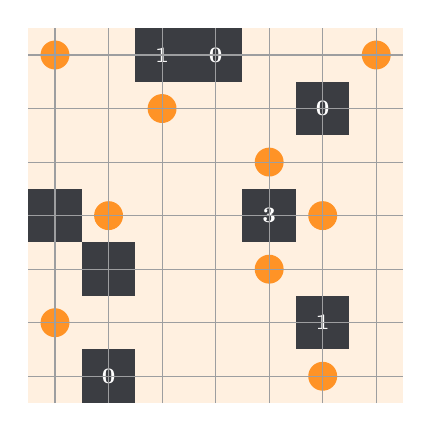
\begin{tikzpicture}[scale=.68]
\fill[orange!12] (-.5,.5) rectangle (6.5,-6.5);
\fill[ink!90] (2-.5,-0-.5) rectangle (2+.5,-0+.5);
\node[white,font=\footnotesize\bfseries] at (2,-0) {1};
\fill[ink!90] (3-.5,-0-.5) rectangle (3+.5,-0+.5);
\node[white,font=\footnotesize\bfseries] at (3,-0) {0};
\fill[ink!90] (5-.5,-1-.5) rectangle (5+.5,-1+.5);
\node[white,font=\footnotesize\bfseries] at (5,-1) {0};
\fill[ink!90] (0-.5,-3-.5) rectangle (0+.5,-3+.5);
\fill[ink!90] (4-.5,-3-.5) rectangle (4+.5,-3+.5);
\node[white,font=\footnotesize\bfseries] at (4,-3) {3};
\fill[ink!90] (1-.5,-4-.5) rectangle (1+.5,-4+.5);
\fill[ink!90] (5-.5,-5-.5) rectangle (5+.5,-5+.5);
\node[white,font=\footnotesize\bfseries] at (5,-5) {1};
\fill[ink!90] (1-.5,-6-.5) rectangle (1+.5,-6+.5);
\node[white,font=\footnotesize\bfseries] at (1,-6) {0};
\fill[orange!85] (0,-0) circle (.27);
\fill[orange!85] (6,-0) circle (.27);
\fill[orange!85] (2,-1) circle (.27);
\fill[orange!85] (4,-2) circle (.27);
\fill[orange!85] (1,-3) circle (.27);
\fill[orange!85] (5,-3) circle (.27);
\fill[orange!85] (4,-4) circle (.27);
\fill[orange!85] (0,-5) circle (.27);
\fill[orange!85] (5,-6) circle (.27);
\draw[ink!45] (-.5,.5) grid (6.5,-6.5);
\end{tikzpicture}

\caption{Bàn $7\times7$, mức easy, seed 70097 và lời giải do CSP tìm được.
Ô đen là tường, hình tròn là bóng đèn.}
\end{figure}

\subsection{Tạo dữ liệu đầu vào}
Bàn được sinh theo seed, nên cùng seed luôn cho cùng một bàn. Có ba mức
easy, normal và hard, khác nhau ở tỉ lệ tường $\rho$. Bàn $n\times n$ có
$M=\operatorname{round}(\rho n^2)$ ô tường:
\begin{center}\small
\begin{tabular}{@{}lrrrrr@{}}\toprule
Mức & $\rho$ & $7\times7$ & $10\times10$ & $14\times14$ & $25\times25$\\\midrule
easy   & 16\%   & 8 & 16 & 31 & 100\\
normal & 10.5\% & 5 & 10 & 21 & 66\\
hard   & 5.5\%  & 3 & 6 & 11 & 34\\
\bottomrule\end{tabular}
\end{center}
Các bước sinh bàn (\path{light_up_problem/generator/generate.py}):
\begin{enumerate}
\item Chọn ngẫu nhiên $M$ vị trí làm tường.
\item Lần lượt đặt bóng vào một ô trắng còn tối cho tới khi mọi ô đều sáng.
Tập bóng này là một lời giải mẫu.
\item Ghi số lên tường bằng số bóng kề trong lời giải mẫu, để khoảng 25\% số
tường không ghi số. Cuối cùng kiểm tra lại lời giải mẫu với luật.
\end{enumerate}
Vì bàn được dựng từ một lời giải nên chắc chắn có nghiệm. Solver không được
biết lời giải mẫu. Nhóm có tham khảo cách đánh giá độ khó theo kỹ thuật suy luận
của Dekker~\cite{akari-difficulty}, nhưng chưa áp dụng; nhãn easy/normal/hard
hiện chỉ phản ánh số tường, và chương trình chưa kiểm tra bàn có nghiệm duy nhất.

\subsection{Giải thuật tìm kiếm mù}
\subsubsection*{Depth-First Search (DFS)}
Ở mỗi bước, DFS lấy ô tối đầu tiên theo thứ tự hàng rồi cột và thử lần lượt
các vị trí có thể đặt bóng để chiếu ô đó. Một vị trí bị bỏ nếu bóng chiếu vào
bóng khác, làm một tường bị thừa bóng hay không còn đủ chỗ đặt bóng, hoặc làm
một ô tối không còn chỗ nào chiếu tới được. DFS đi sâu ngay vào nhánh hợp lệ
đầu tiên và quay lui khi bế tắc.

\noindent\begin{minipage}{\textwidth}
\begin{lstlisting}
DFS(state):
  if budget exhausted: return LIMIT
  if GOAL(state): return SOLVED(state)
  target = first dark cell in row-major order
  for bulb in legal illuminators(target):
    child = place(bulb)
    if FEASIBLE(child):
      result = DFS(child)
      if solved or limited: return result
    exclude bulb from later sibling choices
  return UNSOLVABLE
\end{lstlisting}
\end{minipage}

Dòng \code{exclude bulb} giúp các nhánh anh em không đặt lại một vị trí đã thử,
tránh việc cùng một tập bóng xuất hiện nhiều lần với thứ tự đặt khác nhau.
Trong code, đệ quy được thay bằng stack tường minh. Thứ tự chọn ô và thứ tự thử
là cố định, DFS không dùng điểm đánh giá nào.

Mỗi bước thêm một bóng nên độ sâu không quá $W$. Nếu mỗi ô tối có tối đa $b$
cách chiếu và lời giải sâu $d$, số trạng thái xấu nhất là $O(b^d)$. Stack chỉ
giữ nhánh hiện tại, nhưng chương trình còn lưu liên kết cha để phát lại các
bước, nên bộ nhớ tăng theo số trạng thái đã sinh.

\subsection{Giải thuật tìm kiếm heuristic}
\subsubsection*{Backtracking với MRV và lan truyền ràng buộc (CSP)}
Ý tưởng là suy ra những gì bắt buộc trước, chỉ đoán khi không suy ra được nữa,
và khi phải đoán thì đoán ở chỗ ít lựa chọn nhất. Cách làm này dựa trên phân
tích của Pulles~\cite{akari-analysis} và bộ giải Borroot/akari~\cite{akari-code}.

\paragraph{Trạng thái và tên các bước.} Dùng thống nhất
\code{state = (bulbs, lit, legal)}: tập bóng đã đặt, tập ô đã sáng và tập vị
trí còn được phép đặt bóng. Gọi $P$ là tập ô trắng, $dark=P\setminus lit$,
$V(i)$ là tập ô nhìn thấy từ $i$ (kể cả $i$), $N(w)$ là tập ô trắng kề tường
$w$, và $k_w$ là số ghi trên tường. Các tập này được lưu bằng bitmask trong code.
\code{PROPAGATE} là bước lan truyền ràng buộc;
\code{SELECT\_MRV\_CHOICES} chọn ràng buộc bằng MRV và trả các nhánh theo thứ
tự gain; \code{GOAL} kiểm tra đủ ba điều kiện thắng.

\paragraph{Lan truyền ràng buộc (CP): \code{PROPAGATE}.} Bước này lặp các luật
sau tới điểm cố định (không còn thay đổi), trước khi chọn nhánh:
\begin{itemize}
\item Tường đã đủ bóng thì cấm đặt bóng ở các ô kề còn lại. Tường còn thiếu $r$
bóng và chỉ còn đúng $r$ ô kề đặt được thì đặt bóng ở cả $r$ ô đó.
\item Ô tối chỉ còn một vị trí có thể chiếu tới thì đặt bóng ở vị trí đó.
Mỗi bóng mới làm cấm các ô khác trên đường sáng của nó.
\item Nếu đặt bóng ở một ô làm một tường số không thể đủ bóng, ô đó bị cấm.
\end{itemize}
Nếu gặp mâu thuẫn (ô tối không còn nguồn chiếu, tường không thể đủ bóng) thì
nhánh hiện tại bị bỏ.

\paragraph{Chọn ràng buộc bằng MRV: \code{SELECT\_MRV\_CHOICES}.}
Sau \code{PROPAGATE}, nếu chưa tới đích, MRV (Minimum Remaining Values) so
sánh số lựa chọn của hai loại ràng buộc trên cùng trạng thái:
\begin{itemize}
\item \textbf{Tường số $w$:} số bóng còn thiếu là
$r=k_w-|N(w)\cap bulbs|$; tập ô kề còn được phép đặt là
$U(w)=N(w)\cap legal$, có $u=|U(w)|$ phần tử. Với $r>0$, điểm là
\[
 m_{\mathrm{wall}}(w)=\binom{u}{r}.
\]
Mỗi lựa chọn đặt đúng $r$ bóng vào một tổ hợp của $U(w)$ và cấm các ô kề
không được chọn. Tường đã đủ bóng ($r=0$) không tham gia MRV; $r<0$ hoặc
$r>u$ là mâu thuẫn được phát hiện trong \code{PROPAGATE}.
\item \textbf{Ô tối $i$:} tập nguồn chiếu còn được phép là
$C(i)=V(i)\cap legal$. Điểm là
\[
 m_{\mathrm{dark}}(i)=|C(i)|.
\]
Mỗi lựa chọn đặt một bóng tại một nguồn chiếu trong $C(i)$; $C(i)=\varnothing$
là mâu thuẫn. Tập $legal$ đã loại các ô bị CP cấm, không chỉ xét ô có bóng hay chưa.
\end{itemize}
Chọn ràng buộc có điểm nhỏ nhất trong cả hai nhóm; bằng điểm thì ưu tiên
tường. Trong cùng loại, giữ phần tử gặp trước theo thứ tự duyệt của code.
Ví dụ, tường thiếu $r=2$ bóng và còn $u=3$ ô kề có điểm $3$; ô tối có hai
nguồn chiếu có điểm $2$, nên chọn ô tối. Nếu ô tối cũng có điểm $3$ thì chọn
tường. Điểm $\binom{u}{r}$ được tính \emph{trước} khi sinh và loại các tổ hợp
có bóng chiếu nhau, nên không nhất thiết bằng số nhánh thực tế còn lại.

\paragraph{Sắp thứ tự thử bằng gain.} Sau khi MRV chọn ràng buộc, gọi $A$ là
tập bóng mới của một nhánh: một bóng nếu chọn ô tối, hoặc $r$ bóng nếu chọn
tường. Điểm chiếu sáng thêm là
\[
 gain(A)=\left|\left(\bigcup_{b\in A}V(b)\right)\cap dark\right|
        =|lit_{\mathrm{child}}\setminus lit|.
\]
Lấy hợp trước khi đếm để một ô được nhiều bóng chiếu vẫn chỉ tính một lần.
Thử nhánh có gain lớn trước; bằng gain giữ thứ tự sinh ban đầu. Gain được tính
ngay sau khi đặt $A$, \emph{trước CP của trạng thái con}; không cộng gain vào
điểm MRV và không dùng nó để chọn giữa tường với ô tối.

Ví dụ thực từ bàn $7\times7$ easy, seed 70098: sau CP ở gốc, ô tối
$(6,7)$ có hai nguồn chiếu $(7,7)$ và $(5,7)$ (tọa độ hàng, cột tính từ 1).
Gain tương ứng là $7$ và $6$, nên thử $(7,7)$ trước
(Hình~\ref{fig:lightup-gain-70098}).

\begin{figure}[H]
\centering
\begingroup
\colorlet{blue}{pipeblue}
\colorlet{red}{reject}
\begin{subfigure}[t]{.46\textwidth}
\centering
\scalebox{1.55}{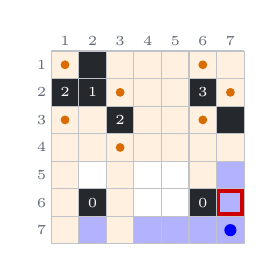
\begin{tikzpicture}[x=.35cm,y=-.35cm,font=\tiny]
% Snapshot after root CP: 7x7 easy, seed 70098; coordinates below are zero-based.
\foreach \c/\r in {0/0,2/0,3/0,4/0,5/0,6/0,2/1,3/1,4/1,6/1,0/2,1/2,3/2,4/2,5/2,0/3,1/3,2/3,3/3,4/3,5/3,6/3,0/4,2/4,5/4,0/5,2/5,0/6,2/6}{\fill[orange!12] (\c,\r) rectangle ++(1,1);}
\foreach \c/\r in {6/4,6/5,1/6,3/6,4/6,5/6,6/6}{\fill[blue!30] (\c,\r) rectangle ++(1,1);}
\foreach \c/\r/\n in {1/0/-1,0/1/2,1/1/1,5/1/3,2/2/2,6/2/-1,1/5/0,5/5/0}{
  \fill[ink] (\c,\r) rectangle ++(1,1);
  \ifnum\n>-1\node[white] at (\c+.5,\r+.5) {\n};\fi}
\foreach \i in {0,...,7}{
  \draw[muted!40,thin] (\i,0)--(\i,7);
  \draw[muted!40,thin] (0,\i)--(7,\i);}
\foreach \c/\r in {0/0,5/0,2/1,6/1,0/2,5/2,2/3}{\fill[orange!85!black] (\c+.5,\r+.5) circle (.16);}
\fill[blue] (6.5,6.5) circle (.22);
\draw[red!80!black,very thick] (6.08,5.08) rectangle (6.92,5.92);
\foreach \i in {0,...,6}{
  \pgfmathtruncatemacro{\labelnum}{\i+1}
  \node[muted] at (\i+.5,-.35) {\labelnum};
  \node[muted] at (-.35,\i+.5) {\labelnum};}
\end{tikzpicture}
}
\caption{Đặt bóng tại $(7,7)$: gain $=7$.}
\end{subfigure}\hfill
\begin{subfigure}[t]{.46\textwidth}
\centering
\scalebox{1.55}{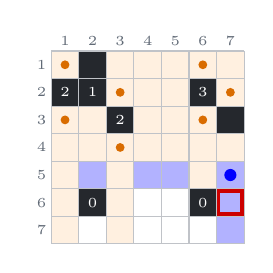
\begin{tikzpicture}[x=.35cm,y=-.35cm,font=\tiny]
% Snapshot after root CP: 7x7 easy, seed 70098; coordinates below are zero-based.
\foreach \c/\r in {0/0,2/0,3/0,4/0,5/0,6/0,2/1,3/1,4/1,6/1,0/2,1/2,3/2,4/2,5/2,0/3,1/3,2/3,3/3,4/3,5/3,6/3,0/4,2/4,5/4,0/5,2/5,0/6,2/6}{\fill[orange!12] (\c,\r) rectangle ++(1,1);}
\foreach \c/\r in {1/4,3/4,4/4,6/4,6/5,6/6}{\fill[blue!30] (\c,\r) rectangle ++(1,1);}
\foreach \c/\r/\n in {1/0/-1,0/1/2,1/1/1,5/1/3,2/2/2,6/2/-1,1/5/0,5/5/0}{
  \fill[ink] (\c,\r) rectangle ++(1,1);
  \ifnum\n>-1\node[white] at (\c+.5,\r+.5) {\n};\fi}
\foreach \i in {0,...,7}{
  \draw[muted!40,thin] (\i,0)--(\i,7);
  \draw[muted!40,thin] (0,\i)--(7,\i);}
\foreach \c/\r in {0/0,5/0,2/1,6/1,0/2,5/2,2/3}{\fill[orange!85!black] (\c+.5,\r+.5) circle (.16);}
\fill[blue] (6.5,4.5) circle (.22);
\draw[red!80!black,very thick] (6.08,5.08) rectangle (6.92,5.92);
\foreach \i in {0,...,6}{
  \pgfmathtruncatemacro{\labelnum}{\i+1}
  \node[muted] at (\i+.5,-.35) {\labelnum};
  \node[muted] at (-.35,\i+.5) {\labelnum};}
\end{tikzpicture}
}
\caption{Đặt bóng tại $(5,7)$: gain $=6$.}
\end{subfigure}
\endgroup
\caption{Ví dụ thực từ bàn $7\times7$ easy, seed 70098, sau CP ở gốc và trước
CP của con. Viền đỏ đánh dấu ô tối $(6,7)$; chấm cam là bóng đã đặt, chấm xanh
là bóng thử. Nền cam nhạt là ô đã sáng, nền xanh là ô mới sáng dùng để tính gain.
Tọa độ hàng và cột tính từ 1.}
\label{fig:lightup-gain-70098}
\end{figure}

Khi chọn nguồn chiếu, các nhánh sau cấm các nguồn đã thử ở nhánh trước:
nhánh thứ hai đặt tại $(5,7)$ đồng thời cấm $(7,7)$. Các nhánh vì thế không
lặp cùng tập bóng theo thứ tự đặt khác nhau. Với tường, tổ hợp không hợp lệ
bị loại trước khi xếp gain; các mâu thuẫn còn lại được CP của con kiểm tra.

\paragraph{Quay lui: \code{BACKTRACK\_MRV\_CP}.} Mã giả dùng cùng tên các
bước ở trên. \code{SELECT\_MRV\_CHOICES} trả các trạng thái con đã áp dụng
lựa chọn và điều kiện cấm của từng nhánh, xếp theo gain giảm dần.

\noindent\begin{minipage}{\textwidth}
\begin{lstlisting}
BACKTRACK_MRV_CP(state):
  if budget exhausted: return LIMIT
  state, ok = PROPAGATE(state)
  if not ok: return UNSOLVABLE
  if GOAL(state): return SOLVED(state)
  checkpoint = state
  choices = SELECT_MRV_CHOICES(checkpoint)
  for child in choices:  # descending gain, before child CP
    result = BACKTRACK_MRV_CP(child)
    if result is SOLVED or LIMIT: return result
    state = checkpoint
  return UNSOLVABLE
\end{lstlisting}
\end{minipage}

Checkpoint giữ đủ \code{(bulbs, lit, legal)} sau CP của nút cha. Khi quay lui,
khôi phục cả ba tập trước khi thử nhánh kế tiếp. Code dùng stack tường minh
thay cho đệ quy; \code{PROPAGATE} tương ứng \code{propagate}, còn
\code{SELECT\_MRV\_CHOICES} tương ứng \code{select\_mrv\_choices} trong
\code{algorithms/search.py}. Mã giả gom các trường hợp dừng do tài nguyên
thành \code{LIMIT}; code kiểm tra giới hạn trong quá trình duyệt, và trong
CP khi bật trace.

Trường hợp xấu nhất CSP vẫn tốn thời gian hàm mũ. CP giúp giảm mạnh số nhánh
nhưng làm mỗi nút tốn công hơn, vì phải lặp các luật suy luận. Một nút CSP có
thể đặt nhiều bóng cùng lúc, nên số nút của CSP và DFS không tương ứng với cùng
một lượng công việc. Cả hai giải thuật chỉ bỏ những nhánh chắc chắn không có
nghiệm, nên sẽ tìm được lời giải nếu đủ thời gian.

\subsection{Hiện thực và minh họa từng bước}
Package \code{light\_up\_problem} gồm \code{core/} (luật và cấu trúc bàn),
\code{generator/} (sinh bàn), \code{algorithms/search.py} (giải thuật),
\code{ui/app.py} (giao diện pygame-ce và pygame-gui) và \code{benchmark/} (đo).
Solver chạy trong một worker riêng để giao diện không bị đứng.

\begin{itemize}
\item \textbf{Chơi tay:} click trái để đặt hoặc bỏ bóng, click phải để đánh dấu
ô không đặt bóng, rồi bấm kiểm tra lời giải.
\item \textbf{Xem giải thuật chạy:} chọn DFS hoặc CSP rồi bấm Start Search.
Có Pause/Resume, hai mũi tên để đi tới hoặc lui từng bước, và ba tốc độ
2, 8, 30 bước mỗi giây.
\item DFS hiện ô đang xét, bóng vừa đặt và lúc quay lui. CSP hiện thêm các bóng
được suy ra, các ô bị cấm (dấu $\times$) và việc khôi phục khi quay lui.
\item Nút \textbf{Compare DFS and CSP} chạy cả hai giải thuật một lần trên bàn
đang mở và hiện thời gian, bộ nhớ, số nút.
\end{itemize}

\subsection{Kết quả thực nghiệm}
Nhóm đo trên 4 kích thước, 3 mức và 5 seed cho mỗi cấu hình, tức 60 bàn khác
nhau. Mỗi bàn được giải một lần bằng mỗi giải thuật, tổng cộng 120 lượt. Mỗi
lượt chạy trong một process mới, các lượt chạy lần lượt và thứ tự hai giải thuật
được đảo ở các seed liên tiếp. Seed dùng cho từng cấu hình:
\begin{center}\small
\begin{tabular}{@{}rlll@{}}\toprule
Cỡ & easy & normal & hard\\\midrule
7 & 70097--70101 & 70194--70198 & 70291--70295\\
10 & 100097--100101 & 100194--100198 & 100291--100295\\
14 & 140097--140101 & 140194--140198 & 140291--140295\\
25 & 250097--250101 & 250194--250198 & 250291--250295\\
\bottomrule\end{tabular}
\end{center}

Mỗi lượt giới hạn 30 giây, 500.000 nút mở rộng và 512 MiB bộ nhớ. Lượt vượt
giới hạn được ghi là TIMEOUT, NODE\_LIMIT hoặc MEMORY\_LIMIT, không bị tính là
vô nghiệm. Thời gian đo bằng \code{perf\_counter} quanh solver, không tính thời
gian sinh bàn hay khởi động process. Bộ nhớ là đỉnh cấp phát của Python đo bằng
\code{tracemalloc}, không phải RAM của cả process. Mọi lời giải đều được kiểm tra
lại bằng \code{is\_goal\_state()}. Số liệu thô nằm ở
\path{docs/benchmarks/2026-10-31-lightup-dfs-csp.csv}.

\begin{center}\small
\begin{tabular}{@{}lrrrr@{}}
\toprule
Giải thuật & SOLVED & TIMEOUT & NODE\_LIMIT & MEMORY\_LIMIT\\
\midrule
DFS & 52 & 8 & 0 & 0\\
CSP & 60 & 0 & 0 & 0\\
\bottomrule
\end{tabular}
\end{center}
% Raw CSV: docs/benchmarks/2026-10-31-lightup-dfs-csp.csv.
% Arithmetic means; seconds/memory/nodes include TIMEOUT, bulbs use SOLVED only.
\begin{table}[H]
\centering\scriptsize
\setlength{\tabcolsep}{4pt}
\begin{tabular}{@{}rllcrrrr@{}}
\toprule
Cỡ & Mức & Giải thuật & Giải được & Thời gian (s) & Bộ nhớ (KiB) & Số nút & Số bóng\\
\midrule
7 & easy & DFS & 5/5 & 0.0102 & 27.1 & 30.6 & 8.4\\
7 & easy & CSP & 5/5 & 0.0078 & 25.1 & 4.0 & 8.4\\
\addlinespace[2pt]
7 & normal & DFS & 5/5 & 0.0067 & 26.8 & 9.2 & 7.6\\
7 & normal & CSP & 5/5 & 0.0103 & 29.1 & 6.2 & 7.2\\
\addlinespace[2pt]
7 & hard & DFS & 5/5 & 0.0072 & 27.3 & 8.4 & 7.4\\
7 & hard & CSP & 5/5 & 0.0105 & 30.5 & 6.4 & 6.2\\
\addlinespace[2pt]
10 & easy & DFS & 5/5 & 0.0360 & 58.7 & 51.6 & 15.4\\
10 & easy & CSP & 5/5 & 0.0280 & 56.0 & 7.8 & 13.8\\
\addlinespace[2pt]
10 & normal & DFS & 5/5 & 0.0280 & 62.6 & 40.2 & 13.0\\
10 & normal & CSP & 5/5 & 0.0312 & 62.2 & 8.8 & 11.6\\
\addlinespace[2pt]
10 & hard & DFS & 5/5 & 0.0230 & 62.4 & 12.4 & 11.4\\
10 & hard & CSP & 5/5 & 0.0314 & 67.7 & 9.8 & 10.0\\
\addlinespace[2pt]
14 & easy & DFS & 5/5 & 0.9070 & 228.9 & 983.4 & 26.2\\
14 & easy & CSP & 5/5 & 0.0947 & 108.3 & 12.4 & 24.4\\
\addlinespace[2pt]
14 & normal & DFS & 5/5 & 1.3044 & 375.7 & 2\,020.2 & 21.6\\
14 & normal & CSP & 5/5 & 0.1033 & 123.7 & 16.0 & 20.0\\
\addlinespace[2pt]
14 & hard & DFS & 5/5 & 0.0858 & 126.2 & 24.0 & 18.6\\
14 & hard & CSP & 5/5 & 0.1177 & 134.3 & 14.6 & 15.2\\
\addlinespace[2pt]
25 & easy & DFS & 2/5 & 23.7947 & 2192.9 & 8\,678.4 & 73.0\\
25 & easy & CSP & 5/5 & 2.1056 & 579.9 & 96.2 & 67.8\\
\addlinespace[2pt]
25 & normal & DFS & 1/5 & 24.2972 & 3522.0 & 13\,406.6 & 58.0\\
25 & normal & CSP & 5/5 & 1.0444 & 693.0 & 33.8 & 52.6\\
\addlinespace[2pt]
25 & hard & DFS & 4/5 & 7.7500 & 1268.7 & 2\,407.8 & 41.0\\
25 & hard & CSP & 5/5 & 1.0463 & 872.3 & 33.6 & 35.2\\
\bottomrule
\end{tabular}
\caption{Light Up: trung bình cộng (mean) trên 5 seed của mỗi cấu hình.
Thời gian, đỉnh bộ nhớ Python và số nút tính cả lượt TIMEOUT: thời gian là
thời lượng chạy tới lúc dừng, không phải thời gian giải xong. Số bóng chỉ lấy
trung bình các lượt SOLVED, với số mẫu ở cột Giải được. Kết quả từng bàn ở phụ lục.}
\label{tab:lightup-dfs-csp-vi}
\end{table}

\subsection{Nhận xét}
\paragraph{Số bàn giải được và số nút.} CSP giải được 60/60 bàn, DFS giải
được 52/60. Tám lượt TIMEOUT đều của DFS, ở bàn $25\times25$; không lượt nào
chạm giới hạn nút hay bộ nhớ. Tại $25\times25$ normal, DFS mở trung bình
13\,406.6 nút so với 33.8 nút của CSP. Ở cỡ 25, CSP mở trung bình 33.6--96.2
nút tùy nhãn. CP có thể suy ra nhiều bóng trong một nút, nên các số này không
đại diện cùng lượng công việc giữa hai giải thuật.

\paragraph{Thời gian.} Trong 52 bàn cả hai cùng giải được, CSP nhanh hơn ở
15 bàn, DFS nhanh hơn ở 37 bàn. Đây là số đếm theo từng cặp, khác với trung
bình theo cấu hình trong Bảng~\ref{tab:lightup-dfs-csp-vi}. Với bàn nhỏ,
chi phí lặp các luật CP có thể khiến CSP chậm hơn DFS; tuy nhiên CSP có mean
thời gian thấp hơn DFS ở $7\times7$ easy và $10\times10$ easy.
Tại $14\times14$ easy, mean DFS/CSP là 0.9070/0.0947 giây, tỉ số khoảng 9.6;
ở normal là 1.3044/0.1033 giây, tỉ số khoảng 12.6. Một số lượt DFS dài làm
mean tăng rõ rệt, nên không suy rộng các tỉ số này cho mọi seed.
Ở $25\times25$, CSP có mean 1.0444--2.1056 giây; mean thời lượng lượt chạy DFS
là 7.7500--24.2972 giây, có tính các lượt bị dừng sau 30 giây. Vì có TIMEOUT,
tỉ số thời lượng trung bình ở các nhóm này không phải tỉ số thời gian giải
xong trên cùng tập bàn.

\paragraph{Bộ nhớ và số bóng.} Ở cỡ 7 và 10, mean đỉnh bộ nhớ Python của
hai giải thuật khá gần nhau. Tại $25\times25$ easy và normal, mean DFS/CSP
lần lượt là 2192.9/579.9 KiB và 3522.0/693.0 KiB, tức khoảng 3.8 và 5.1 lần;
ở hard tỉ số khoảng 1.5 lần. DFS phải giữ nhiều trạng thái đã sinh để phát
lại đường đi. Cột Số bóng là mean riêng trên các lượt SOLVED: khi số lượt giải
được khác nhau, hai mean có thể dựa trên tập seed khác nhau. Trong 52 cặp
cùng giải được, CSP dùng ít bóng hơn ở 39 bàn; cả hai không bảo đảm tối ưu số bóng.

\paragraph{Hạn chế.} Mỗi cấu hình mới có 5 seed; mean nhạy với các lượt chạy
dài và các lượt bị giới hạn. Nhãn độ khó chỉ dựa trên số tường; ở cỡ 14 và 25,
mean thời lượng DFS ở hard thấp hơn easy và normal. Chương trình chưa kiểm
tra tính duy nhất của lời giải và chưa đo riêng tác dụng của MRV, gain và CP.
Các lượt đo cũ ngày 25/10 dùng generator trước đó được lưu riêng,
không trộn vào bảng thực nghiệm mới.


\section*{Kết luận}
\addcontentsline{toc}{section}{Kết luận}
Nhóm đã hiện thực hai trò chơi Pipes và Light Up bằng Python 3. Mỗi trò chơi
có chế độ chơi tay, chế độ xem giải thuật chạy từng bước, và hai giải thuật:
một giải thuật mù (DFS) và một giải thuật có heuristic.

\begin{itemize}
\item \textbf{Pipes:} DFS và Greedy Best-First đều giải được cả 9 bàn trong vài
chục mili giây. Vì cắt tỉa đã loại gần hết hướng sai, hai giải thuật chạy nhanh
gần như nhau; Greedy dùng ít bộ nhớ hơn trên bộ thử này.
\item \textbf{Light Up:} CSP (backtracking với MRV và lan truyền ràng buộc) giải
được 60/60 bàn, DFS giải được 52/60. Ở bàn $25\times25$, thời gian trung bình
của CSP khoảng 1.04--2.11 giây tùy nhãn; DFS có 8 lượt bị dừng sau 30 giây.
Các giá trị trung bình trong bảng tính cả lượt TIMEOUT, nên không coi thời
lượng lượt bị dừng là thời gian giải xong.
\end{itemize}

Bài học chính của nhóm là heuristic không phải lúc nào cũng làm giải thuật nhanh
hơn: nó có ích khi không gian tìm kiếm đủ lớn, còn ở bài dễ thì chi phí tính
heuristic có thể lớn hơn phần tiết kiệm được. Hướng phát triển tiếp theo là thêm
bàn khó và bàn vô nghiệm, đo nhiều seed hơn, kiểm tra tính duy nhất của lời giải
Light Up và đo riêng tác dụng của từng kỹ thuật cắt tỉa, MRV và CP.

\clearpage
\section*{Phụ lục: Kết quả theo từng input Light Up}
\addcontentsline{toc}{section}{Phụ lục: Kết quả theo từng input Light Up}
Mỗi dòng là một bàn, giải một lần bằng mỗi giải thuật. Thời gian tính bằng
giây, bộ nhớ là đỉnh cấp phát Python tính bằng KiB. Cột TT DFS ghi S (SOLVED)
hoặc T (TIMEOUT); với lượt T, thời gian là lúc bị dừng. CSP giải được tất cả
các bàn. Số liệu đo ngày 31/10/2026.

\begin{table}[H]\centering\small
\setlength{\tabcolsep}{4pt}
\begin{tabular*}{\textwidth}{@{\extracolsep{\fill}}rlrcrrrr@{}}\toprule
 & & & & \multicolumn{2}{c}{DFS} & \multicolumn{2}{c}{CSP}\\
Cỡ & Nhãn & Seed & TT DFS & Giây & KiB & Giây & KiB\\\midrule
7 & easy & 70097 & S & 0.0075 & 24.9 & 0.0115 & 25.4\\
7 & easy & 70098 & S & 0.0084 & 25.4 & 0.0057 & 24.8\\
7 & easy & 70099 & S & 0.0236 & 36.7 & 0.0066 & 25.2\\
7 & easy & 70100 & S & 0.0057 & 24.8 & 0.0062 & 24.8\\
7 & easy & 70101 & S & 0.0060 & 23.8 & 0.0091 & 25.5\\
7 & normal & 70194 & S & 0.0066 & 27.1 & 0.0103 & 28.6\\
7 & normal & 70195 & S & 0.0063 & 26.7 & 0.0106 & 29.4\\
7 & normal & 70196 & S & 0.0070 & 26.8 & 0.0104 & 29.0\\
7 & normal & 70197 & S & 0.0063 & 26.6 & 0.0098 & 29.8\\
7 & normal & 70198 & S & 0.0071 & 26.9 & 0.0102 & 28.5\\
7 & hard & 70291 & S & 0.0079 & 27.2 & 0.0109 & 30.0\\
7 & hard & 70292 & S & 0.0079 & 27.3 & 0.0108 & 30.9\\
7 & hard & 70293 & S & 0.0064 & 27.6 & 0.0095 & 30.6\\
7 & hard & 70294 & S & 0.0065 & 27.3 & 0.0107 & 30.5\\
7 & hard & 70295 & S & 0.0074 & 27.1 & 0.0106 & 30.3\\
10 & easy & 100097 & S & 0.0189 & 55.1 & 0.0222 & 54.7\\
10 & easy & 100098 & S & 0.0229 & 55.9 & 0.0244 & 55.0\\
10 & easy & 100099 & S & 0.0203 & 54.9 & 0.0313 & 56.2\\
10 & easy & 100100 & S & 0.0495 & 59.1 & 0.0288 & 56.9\\
10 & easy & 100101 & S & 0.0685 & 68.2 & 0.0331 & 57.0\\
10 & normal & 100194 & S & 0.0201 & 59.0 & 0.0323 & 62.8\\
10 & normal & 100195 & S & 0.0204 & 59.0 & 0.0309 & 61.4\\
10 & normal & 100196 & S & 0.0230 & 61.2 & 0.0279 & 61.1\\
10 & normal & 100197 & S & 0.0218 & 60.0 & 0.0341 & 63.6\\
10 & normal & 100198 & S & 0.0548 & 73.5 & 0.0305 & 61.8\\
10 & hard & 100291 & S & 0.0238 & 61.6 & 0.0334 & 67.8\\
10 & hard & 100292 & S & 0.0237 & 62.4 & 0.0284 & 66.2\\
10 & hard & 100293 & S & 0.0229 & 62.4 & 0.0348 & 67.2\\
10 & hard & 100294 & S & 0.0223 & 62.3 & 0.0293 & 68.2\\
10 & hard & 100295 & S & 0.0223 & 63.3 & 0.0314 & 69.2\\
\bottomrule\end{tabular*}
\caption{Kết quả từng input Light Up, cỡ 7 và 10.}
\end{table}
\clearpage
\begin{table}[H]\centering\small
\setlength{\tabcolsep}{4pt}
\begin{tabular*}{\textwidth}{@{\extracolsep{\fill}}rlrcrrrr@{}}\toprule
 & & & & \multicolumn{2}{c}{DFS} & \multicolumn{2}{c}{CSP}\\
Cỡ & Nhãn & Seed & TT DFS & Giây & KiB & Giây & KiB\\\midrule
14 & easy & 140097 & S & 3.5735 & 593.5 & 0.1642 & 110.4\\
14 & easy & 140098 & S & 0.4546 & 176.2 & 0.0883 & 110.9\\
14 & easy & 140099 & S & 0.2330 & 135.3 & 0.0680 & 105.0\\
14 & easy & 140100 & S & 0.0701 & 110.1 & 0.0801 & 106.1\\
14 & easy & 140101 & S & 0.2036 & 129.3 & 0.0730 & 109.1\\
14 & normal & 140194 & S & 0.0596 & 117.3 & 0.0902 & 126.3\\
14 & normal & 140195 & S & 0.8866 & 242.5 & 0.0883 & 122.0\\
14 & normal & 140196 & S & 0.0647 & 116.6 & 0.1030 & 122.4\\
14 & normal & 140197 & S & 5.4386 & 1284.9 & 0.1190 & 123.5\\
14 & normal & 140198 & S & 0.0724 & 117.1 & 0.1160 & 124.2\\
14 & hard & 140291 & S & 0.0815 & 125.2 & 0.1168 & 135.7\\
14 & hard & 140292 & S & 0.0991 & 126.1 & 0.1124 & 134.3\\
14 & hard & 140293 & S & 0.0841 & 126.8 & 0.1159 & 134.6\\
14 & hard & 140294 & S & 0.0809 & 125.8 & 0.1262 & 135.0\\
14 & hard & 140295 & S & 0.0832 & 127.0 & 0.1172 & 132.0\\
25 & easy & 250097 & S & 18.3397 & 2440.6 & 6.7115 & 656.3\\
25 & easy & 250098 & T & 30.0018 & 2495.0 & 0.9558 & 550.6\\
25 & easy & 250099 & T & 30.0001 & 2237.0 & 0.9504 & 562.1\\
25 & easy & 250100 & S & 10.6316 & 1572.3 & 0.9626 & 554.0\\
25 & easy & 250101 & T & 30.0001 & 2219.6 & 0.9475 & 576.4\\
25 & normal & 250194 & S & 1.4799 & 797.0 & 1.0059 & 696.9\\
25 & normal & 250195 & T & 30.0009 & 3583.3 & 0.9933 & 711.0\\
25 & normal & 250196 & T & 30.0002 & 6332.1 & 1.0680 & 697.5\\
25 & normal & 250197 & T & 30.0004 & 4732.9 & 1.1273 & 681.6\\
25 & normal & 250198 & T & 30.0044 & 2164.9 & 1.0274 & 677.9\\
25 & hard & 250291 & S & 0.7432 & 828.5 & 1.0389 & 856.5\\
25 & hard & 250292 & S & 0.7423 & 850.3 & 1.0203 & 879.0\\
25 & hard & 250293 & T & 30.0000 & 1938.4 & 1.0464 & 855.0\\
25 & hard & 250294 & S & 0.7835 & 870.3 & 1.0421 & 902.7\\
25 & hard & 250295 & S & 6.4809 & 1855.9 & 1.0838 & 868.0\\
\bottomrule\end{tabular*}
\caption{Kết quả từng input Light Up, cỡ 14 và 25.}
\end{table}

\clearpage
\begin{thebibliography}{99}
\raggedright
\addcontentsline{toc}{section}{Tài liệu tham khảo}
\bibitem{akari-np} B. McPhail. \emph{Light Up is NP-complete}, 2005.
\url{https://www.mountainvistasoft.com/docs/lightup-is-np-complete.pdf}
\bibitem{akari-difficulty} V. Dekker. \emph{A Difficulty Measure for Light Up Puzzles}.
Luận văn cử nhân, Leiden University, 2015.
\url{https://theses.liacs.nl/pdf/2014-2015Victor-Dekker.pdf}
\bibitem{akari-analysis} B. Pulles. \emph{Analysis of Akari}.
Luận văn cử nhân, Radboud University, 2021; mục 4.1.1 và 4.1.3.
\url{https://www.cs.ru.nl/bachelors-theses/2021/Bram_Pulles___1015194___Analysis_of_Akari.pdf}
\bibitem{akari-code} Borroot. \emph{akari}: mã nguồn bộ giải,
đặc biệt \code{src/tracksolver.py}.
\url{https://github.com/borroot/akari}
\bibitem{akari-rules} Nikoli. \emph{Akari}: luật chơi chính thức.
\url{https://www.nikoli.co.jp/en/puzzles/akari/}
\bibitem{lightup} Puzzle Light Up. Trò chơi trực tuyến và giao diện tham khảo.
\url{https://www.puzzle-light-up.com/}
\bibitem{pipes} Puzzle Pipes. \url{https://www.puzzle-pipes.com/}
\bibitem{aima} S.~J. Russell, P.~Norvig, \emph{Artificial Intelligence: A Modern
Approach}, 4th edition, Pearson, 2021 (chương 3: Tìm kiếm trong không gian
trạng thái; chương 6: Ràng buộc).
\bibitem{pydoc} Python 3 documentation: \code{time}, \code{tracemalloc},
\code{multiprocessing}, \code{heapq}, \code{unittest}.
\url{https://docs.python.org/3/}
\bibitem{pygame} pygame-ce documentation. \url{https://pyga.me/docs/}
\quad pygame\_gui documentation. \url{https://pygame-gui.readthedocs.io/}
\end{thebibliography}

\end{document}
